\begin{figure}[H]
\centering
\begingroup
\newcommand{\triangleneighbors}[1]{%
  \begin{tikzpicture}[x=.62cm,y=.62cm,baseline=(current bounding box.center)]
    \coordinate (a) at (0,0);
    \coordinate (b) at (1,.62);
    \coordinate (c) at (1,-.62);
    \coordinate (v) at (2.05,.20);
    \draw[line width=.6pt] (a)--(b)--(c)--cycle;
    \ifnum#1>0 \draw[densely dashed] (v)--(b);\fi
    \ifnum#1>1 \draw[densely dashed] (v)--(c);\fi
    \ifnum#1>2 \draw[densely dashed] (v)--(a);\fi
    \foreach \root in {a,b,c} {\fill (\root) circle[radius=1.3pt];}
    \draw[fill=white] (v) circle[radius=1.6pt];
  \end{tikzpicture}}
\begin{tabular}{cccc}
\triangleneighbors{0} & \triangleneighbors{1} & \triangleneighbors{2} & \triangleneighbors{3}\\
0 neighbors & 1 neighbor & 2 neighbors & 3 neighbors
\end{tabular}\par\medskip
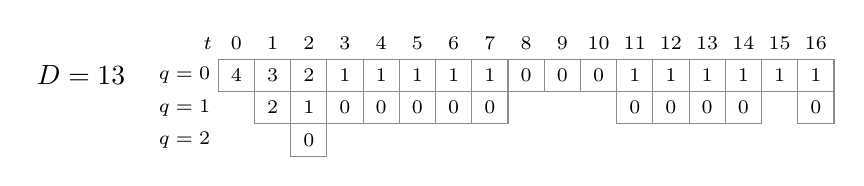
\begin{tikzpicture}[x=.46cm,y=.41cm,baseline=(current bounding box.center)]
\node[anchor=east] at (-2.8,-1) {$D=13$};
\node[anchor=east,font=\scriptsize] at (-.4,0) {$t$};
\node[font=\scriptsize] at (0,0) {$0$};
\node[font=\scriptsize] at (1,0) {$1$};
\node[font=\scriptsize] at (2,0) {$2$};
\node[font=\scriptsize] at (3,0) {$3$};
\node[font=\scriptsize] at (4,0) {$4$};
\node[font=\scriptsize] at (5,0) {$5$};
\node[font=\scriptsize] at (6,0) {$6$};
\node[font=\scriptsize] at (7,0) {$7$};
\node[font=\scriptsize] at (8,0) {$8$};
\node[font=\scriptsize] at (9,0) {$9$};
\node[font=\scriptsize] at (10,0) {$10$};
\node[font=\scriptsize] at (11,0) {$11$};
\node[font=\scriptsize] at (12,0) {$12$};
\node[font=\scriptsize] at (13,0) {$13$};
\node[font=\scriptsize] at (14,0) {$14$};
\node[font=\scriptsize] at (15,0) {$15$};
\node[font=\scriptsize] at (16,0) {$16$};
\node[anchor=east,font=\scriptsize] at (-.45,-1) {$q=0$};
\node[font=\scriptsize,draw=black!45,minimum width=.46cm,minimum height=.41cm,inner sep=0pt] at (0,-1) {$4$};
\node[font=\scriptsize,draw=black!45,minimum width=.46cm,minimum height=.41cm,inner sep=0pt] at (1,-1) {$3$};
\node[font=\scriptsize,draw=black!45,minimum width=.46cm,minimum height=.41cm,inner sep=0pt] at (2,-1) {$2$};
\node[font=\scriptsize,draw=black!45,minimum width=.46cm,minimum height=.41cm,inner sep=0pt] at (3,-1) {$1$};
\node[font=\scriptsize,draw=black!45,minimum width=.46cm,minimum height=.41cm,inner sep=0pt] at (4,-1) {$1$};
\node[font=\scriptsize,draw=black!45,minimum width=.46cm,minimum height=.41cm,inner sep=0pt] at (5,-1) {$1$};
\node[font=\scriptsize,draw=black!45,minimum width=.46cm,minimum height=.41cm,inner sep=0pt] at (6,-1) {$1$};
\node[font=\scriptsize,draw=black!45,minimum width=.46cm,minimum height=.41cm,inner sep=0pt] at (7,-1) {$1$};
\node[font=\scriptsize,draw=black!45,minimum width=.46cm,minimum height=.41cm,inner sep=0pt] at (8,-1) {$0$};
\node[font=\scriptsize,draw=black!45,minimum width=.46cm,minimum height=.41cm,inner sep=0pt] at (9,-1) {$0$};
\node[font=\scriptsize,draw=black!45,minimum width=.46cm,minimum height=.41cm,inner sep=0pt] at (10,-1) {$0$};
\node[font=\scriptsize,draw=black!45,minimum width=.46cm,minimum height=.41cm,inner sep=0pt] at (11,-1) {$1$};
\node[font=\scriptsize,draw=black!45,minimum width=.46cm,minimum height=.41cm,inner sep=0pt] at (12,-1) {$1$};
\node[font=\scriptsize,draw=black!45,minimum width=.46cm,minimum height=.41cm,inner sep=0pt] at (13,-1) {$1$};
\node[font=\scriptsize,draw=black!45,minimum width=.46cm,minimum height=.41cm,inner sep=0pt] at (14,-1) {$1$};
\node[font=\scriptsize,draw=black!45,minimum width=.46cm,minimum height=.41cm,inner sep=0pt] at (15,-1) {$1$};
\node[font=\scriptsize,draw=black!45,minimum width=.46cm,minimum height=.41cm,inner sep=0pt] at (16,-1) {$1$};
\node[anchor=east,font=\scriptsize] at (-.45,-2) {$q=1$};
\node[font=\scriptsize,draw=black!45,minimum width=.46cm,minimum height=.41cm,inner sep=0pt] at (1,-2) {$2$};
\node[font=\scriptsize,draw=black!45,minimum width=.46cm,minimum height=.41cm,inner sep=0pt] at (2,-2) {$1$};
\node[font=\scriptsize,draw=black!45,minimum width=.46cm,minimum height=.41cm,inner sep=0pt] at (3,-2) {$0$};
\node[font=\scriptsize,draw=black!45,minimum width=.46cm,minimum height=.41cm,inner sep=0pt] at (4,-2) {$0$};
\node[font=\scriptsize,draw=black!45,minimum width=.46cm,minimum height=.41cm,inner sep=0pt] at (5,-2) {$0$};
\node[font=\scriptsize,draw=black!45,minimum width=.46cm,minimum height=.41cm,inner sep=0pt] at (6,-2) {$0$};
\node[font=\scriptsize,draw=black!45,minimum width=.46cm,minimum height=.41cm,inner sep=0pt] at (7,-2) {$0$};
\node[font=\scriptsize,draw=black!45,minimum width=.46cm,minimum height=.41cm,inner sep=0pt] at (11,-2) {$0$};
\node[font=\scriptsize,draw=black!45,minimum width=.46cm,minimum height=.41cm,inner sep=0pt] at (12,-2) {$0$};
\node[font=\scriptsize,draw=black!45,minimum width=.46cm,minimum height=.41cm,inner sep=0pt] at (13,-2) {$0$};
\node[font=\scriptsize,draw=black!45,minimum width=.46cm,minimum height=.41cm,inner sep=0pt] at (14,-2) {$0$};
\node[font=\scriptsize,draw=black!45,minimum width=.46cm,minimum height=.41cm,inner sep=0pt] at (16,-2) {$0$};
\node[anchor=east,font=\scriptsize] at (-.45,-3) {$q=2$};
\node[font=\scriptsize,draw=black!45,minimum width=.46cm,minimum height=.41cm,inner sep=0pt] at (2,-3) {$0$};
\end{tikzpicture}
\par\smallskip
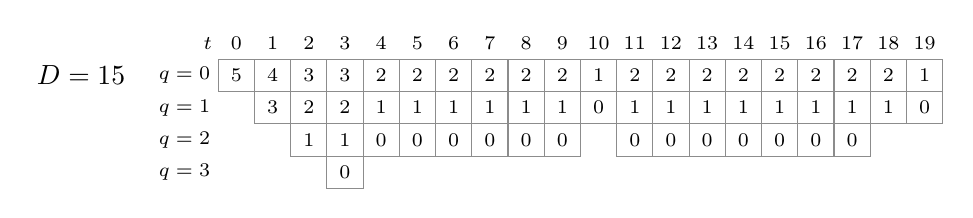
\begin{tikzpicture}[x=.46cm,y=.41cm,baseline=(current bounding box.center)]
\node[anchor=east] at (-2.8,-1) {$D=15$};
\node[anchor=east,font=\scriptsize] at (-.4,0) {$t$};
\node[font=\scriptsize] at (0,0) {$0$};
\node[font=\scriptsize] at (1,0) {$1$};
\node[font=\scriptsize] at (2,0) {$2$};
\node[font=\scriptsize] at (3,0) {$3$};
\node[font=\scriptsize] at (4,0) {$4$};
\node[font=\scriptsize] at (5,0) {$5$};
\node[font=\scriptsize] at (6,0) {$6$};
\node[font=\scriptsize] at (7,0) {$7$};
\node[font=\scriptsize] at (8,0) {$8$};
\node[font=\scriptsize] at (9,0) {$9$};
\node[font=\scriptsize] at (10,0) {$10$};
\node[font=\scriptsize] at (11,0) {$11$};
\node[font=\scriptsize] at (12,0) {$12$};
\node[font=\scriptsize] at (13,0) {$13$};
\node[font=\scriptsize] at (14,0) {$14$};
\node[font=\scriptsize] at (15,0) {$15$};
\node[font=\scriptsize] at (16,0) {$16$};
\node[font=\scriptsize] at (17,0) {$17$};
\node[font=\scriptsize] at (18,0) {$18$};
\node[font=\scriptsize] at (19,0) {$19$};
\node[anchor=east,font=\scriptsize] at (-.45,-1) {$q=0$};
\node[font=\scriptsize,draw=black!45,minimum width=.46cm,minimum height=.41cm,inner sep=0pt] at (0,-1) {$5$};
\node[font=\scriptsize,draw=black!45,minimum width=.46cm,minimum height=.41cm,inner sep=0pt] at (1,-1) {$4$};
\node[font=\scriptsize,draw=black!45,minimum width=.46cm,minimum height=.41cm,inner sep=0pt] at (2,-1) {$3$};
\node[font=\scriptsize,draw=black!45,minimum width=.46cm,minimum height=.41cm,inner sep=0pt] at (3,-1) {$3$};
\node[font=\scriptsize,draw=black!45,minimum width=.46cm,minimum height=.41cm,inner sep=0pt] at (4,-1) {$2$};
\node[font=\scriptsize,draw=black!45,minimum width=.46cm,minimum height=.41cm,inner sep=0pt] at (5,-1) {$2$};
\node[font=\scriptsize,draw=black!45,minimum width=.46cm,minimum height=.41cm,inner sep=0pt] at (6,-1) {$2$};
\node[font=\scriptsize,draw=black!45,minimum width=.46cm,minimum height=.41cm,inner sep=0pt] at (7,-1) {$2$};
\node[font=\scriptsize,draw=black!45,minimum width=.46cm,minimum height=.41cm,inner sep=0pt] at (8,-1) {$2$};
\node[font=\scriptsize,draw=black!45,minimum width=.46cm,minimum height=.41cm,inner sep=0pt] at (9,-1) {$2$};
\node[font=\scriptsize,draw=black!45,minimum width=.46cm,minimum height=.41cm,inner sep=0pt] at (10,-1) {$1$};
\node[font=\scriptsize,draw=black!45,minimum width=.46cm,minimum height=.41cm,inner sep=0pt] at (11,-1) {$2$};
\node[font=\scriptsize,draw=black!45,minimum width=.46cm,minimum height=.41cm,inner sep=0pt] at (12,-1) {$2$};
\node[font=\scriptsize,draw=black!45,minimum width=.46cm,minimum height=.41cm,inner sep=0pt] at (13,-1) {$2$};
\node[font=\scriptsize,draw=black!45,minimum width=.46cm,minimum height=.41cm,inner sep=0pt] at (14,-1) {$2$};
\node[font=\scriptsize,draw=black!45,minimum width=.46cm,minimum height=.41cm,inner sep=0pt] at (15,-1) {$2$};
\node[font=\scriptsize,draw=black!45,minimum width=.46cm,minimum height=.41cm,inner sep=0pt] at (16,-1) {$2$};
\node[font=\scriptsize,draw=black!45,minimum width=.46cm,minimum height=.41cm,inner sep=0pt] at (17,-1) {$2$};
\node[font=\scriptsize,draw=black!45,minimum width=.46cm,minimum height=.41cm,inner sep=0pt] at (18,-1) {$2$};
\node[font=\scriptsize,draw=black!45,minimum width=.46cm,minimum height=.41cm,inner sep=0pt] at (19,-1) {$1$};
\node[anchor=east,font=\scriptsize] at (-.45,-2) {$q=1$};
\node[font=\scriptsize,draw=black!45,minimum width=.46cm,minimum height=.41cm,inner sep=0pt] at (1,-2) {$3$};
\node[font=\scriptsize,draw=black!45,minimum width=.46cm,minimum height=.41cm,inner sep=0pt] at (2,-2) {$2$};
\node[font=\scriptsize,draw=black!45,minimum width=.46cm,minimum height=.41cm,inner sep=0pt] at (3,-2) {$2$};
\node[font=\scriptsize,draw=black!45,minimum width=.46cm,minimum height=.41cm,inner sep=0pt] at (4,-2) {$1$};
\node[font=\scriptsize,draw=black!45,minimum width=.46cm,minimum height=.41cm,inner sep=0pt] at (5,-2) {$1$};
\node[font=\scriptsize,draw=black!45,minimum width=.46cm,minimum height=.41cm,inner sep=0pt] at (6,-2) {$1$};
\node[font=\scriptsize,draw=black!45,minimum width=.46cm,minimum height=.41cm,inner sep=0pt] at (7,-2) {$1$};
\node[font=\scriptsize,draw=black!45,minimum width=.46cm,minimum height=.41cm,inner sep=0pt] at (8,-2) {$1$};
\node[font=\scriptsize,draw=black!45,minimum width=.46cm,minimum height=.41cm,inner sep=0pt] at (9,-2) {$1$};
\node[font=\scriptsize,draw=black!45,minimum width=.46cm,minimum height=.41cm,inner sep=0pt] at (10,-2) {$0$};
\node[font=\scriptsize,draw=black!45,minimum width=.46cm,minimum height=.41cm,inner sep=0pt] at (11,-2) {$1$};
\node[font=\scriptsize,draw=black!45,minimum width=.46cm,minimum height=.41cm,inner sep=0pt] at (12,-2) {$1$};
\node[font=\scriptsize,draw=black!45,minimum width=.46cm,minimum height=.41cm,inner sep=0pt] at (13,-2) {$1$};
\node[font=\scriptsize,draw=black!45,minimum width=.46cm,minimum height=.41cm,inner sep=0pt] at (14,-2) {$1$};
\node[font=\scriptsize,draw=black!45,minimum width=.46cm,minimum height=.41cm,inner sep=0pt] at (15,-2) {$1$};
\node[font=\scriptsize,draw=black!45,minimum width=.46cm,minimum height=.41cm,inner sep=0pt] at (16,-2) {$1$};
\node[font=\scriptsize,draw=black!45,minimum width=.46cm,minimum height=.41cm,inner sep=0pt] at (17,-2) {$1$};
\node[font=\scriptsize,draw=black!45,minimum width=.46cm,minimum height=.41cm,inner sep=0pt] at (18,-2) {$1$};
\node[font=\scriptsize,draw=black!45,minimum width=.46cm,minimum height=.41cm,inner sep=0pt] at (19,-2) {$0$};
\node[anchor=east,font=\scriptsize] at (-.45,-3) {$q=2$};
\node[font=\scriptsize,draw=black!45,minimum width=.46cm,minimum height=.41cm,inner sep=0pt] at (2,-3) {$1$};
\node[font=\scriptsize,draw=black!45,minimum width=.46cm,minimum height=.41cm,inner sep=0pt] at (3,-3) {$1$};
\node[font=\scriptsize,draw=black!45,minimum width=.46cm,minimum height=.41cm,inner sep=0pt] at (4,-3) {$0$};
\node[font=\scriptsize,draw=black!45,minimum width=.46cm,minimum height=.41cm,inner sep=0pt] at (5,-3) {$0$};
\node[font=\scriptsize,draw=black!45,minimum width=.46cm,minimum height=.41cm,inner sep=0pt] at (6,-3) {$0$};
\node[font=\scriptsize,draw=black!45,minimum width=.46cm,minimum height=.41cm,inner sep=0pt] at (7,-3) {$0$};
\node[font=\scriptsize,draw=black!45,minimum width=.46cm,minimum height=.41cm,inner sep=0pt] at (8,-3) {$0$};
\node[font=\scriptsize,draw=black!45,minimum width=.46cm,minimum height=.41cm,inner sep=0pt] at (9,-3) {$0$};
\node[font=\scriptsize,draw=black!45,minimum width=.46cm,minimum height=.41cm,inner sep=0pt] at (11,-3) {$0$};
\node[font=\scriptsize,draw=black!45,minimum width=.46cm,minimum height=.41cm,inner sep=0pt] at (12,-3) {$0$};
\node[font=\scriptsize,draw=black!45,minimum width=.46cm,minimum height=.41cm,inner sep=0pt] at (13,-3) {$0$};
\node[font=\scriptsize,draw=black!45,minimum width=.46cm,minimum height=.41cm,inner sep=0pt] at (14,-3) {$0$};
\node[font=\scriptsize,draw=black!45,minimum width=.46cm,minimum height=.41cm,inner sep=0pt] at (15,-3) {$0$};
\node[font=\scriptsize,draw=black!45,minimum width=.46cm,minimum height=.41cm,inner sep=0pt] at (16,-3) {$0$};
\node[font=\scriptsize,draw=black!45,minimum width=.46cm,minimum height=.41cm,inner sep=0pt] at (17,-3) {$0$};
\node[anchor=east,font=\scriptsize] at (-.45,-4) {$q=3$};
\node[font=\scriptsize,draw=black!45,minimum width=.46cm,minimum height=.41cm,inner sep=0pt] at (3,-4) {$0$};
\end{tikzpicture}
\par\smallskip

\endgroup
\caption{Neighborhoods of an outside vertex at a marked triangle.
For each listed pair $(t,q)$, the entry is the largest retained value of $E$.
A blank cell has no retained triple.}
\label{fig:finite-triangle-profiles}
\end{figure}
